\documentclass[tikz,border=8pt]{standalone}
\usetikzlibrary{shapes.geometric, arrows.meta, positioning, fit, backgrounds}
\usepackage{amsmath,amssymb}

\begin{document}
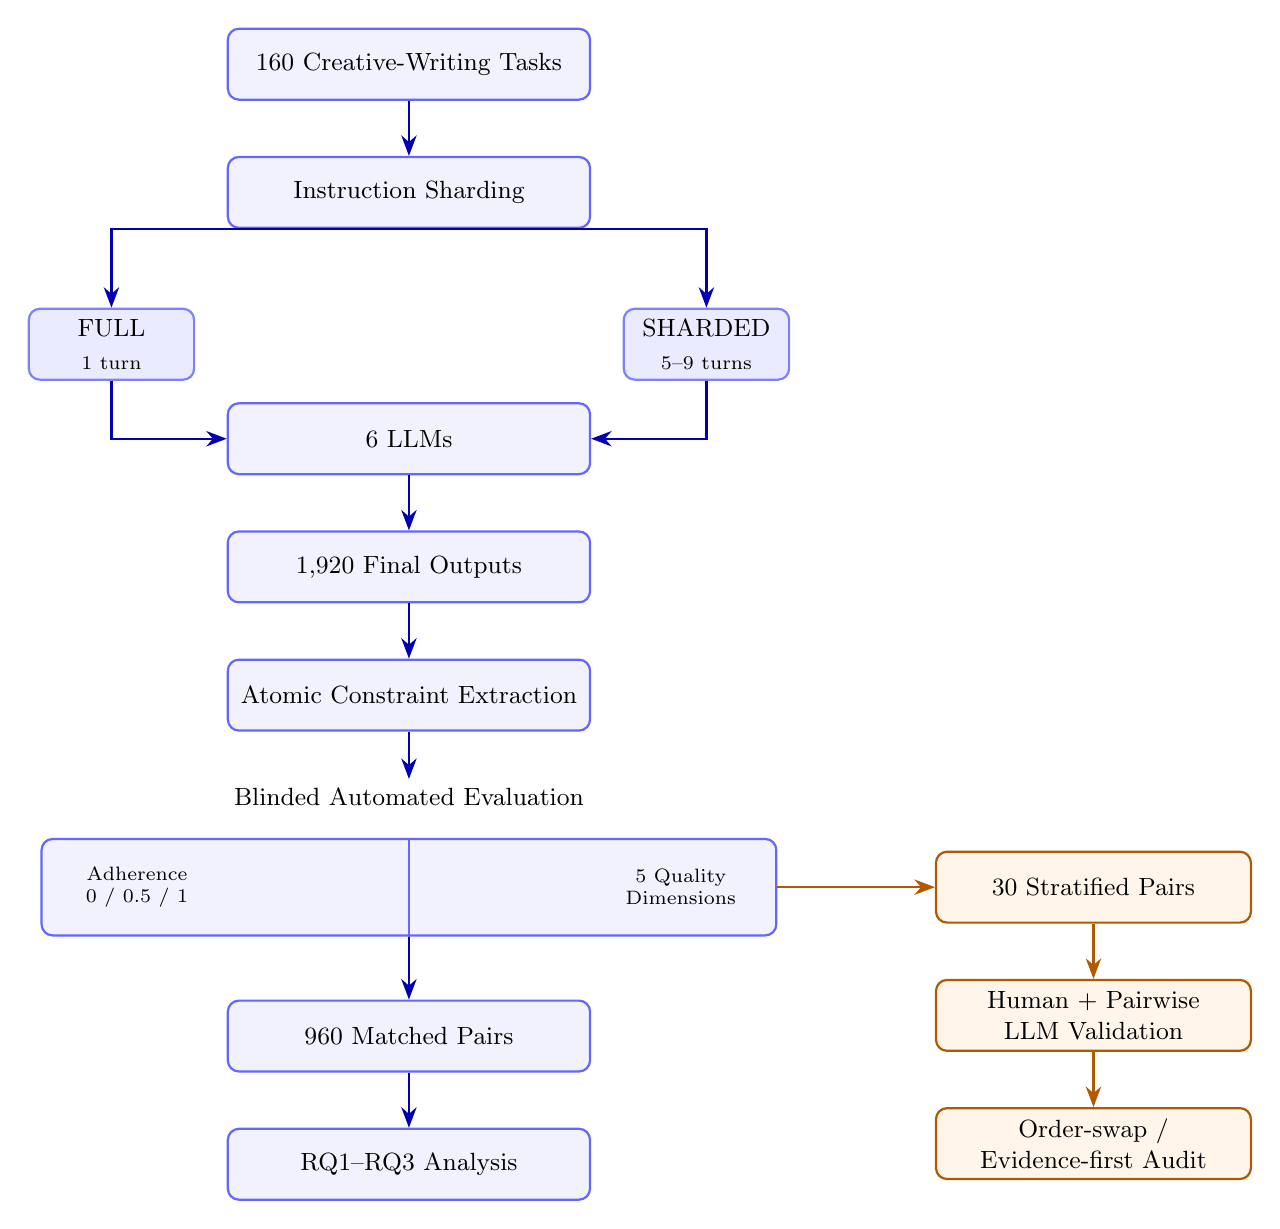
\begin{tikzpicture}[
    node distance=7mm and 9mm,
    box/.style={rectangle, draw=blue!60, fill=blue!5, thick,
        minimum width=4.6cm, minimum height=0.9cm, align=center,
        rounded corners, font=\small},
    condbox/.style={rectangle, draw=blue!50, fill=blue!8, thick,
        minimum width=2.1cm, minimum height=0.9cm, align=center,
        rounded corners, font=\small},
    cellbox/.style={rectangle, draw=none, fill=none,
        minimum width=2.2cm, minimum height=1.0cm, align=center, font=\scriptsize},
    sidebox/.style={rectangle, draw=orange!70!black, fill=orange!8, thick,
        minimum width=4.0cm, minimum height=0.9cm, align=center,
        rounded corners, font=\small},
    arrow/.style={-{Stealth[length=2.6mm]}, thick, draw=blue!70!black},
    sidearrow/.style={-{Stealth[length=2.6mm]}, thick, draw=orange!70!black},
]

% ---- main spine ----
\node (tasks)    [box] {160 Creative-Writing Tasks};
\node (sharding) [box, below=of tasks] {Instruction Sharding};

\node (full)    [condbox, below left=10mm and 4mm of sharding]  {FULL\\[1pt]\scriptsize 1 turn};
\node (sharded) [condbox, below right=10mm and 4mm of sharding] {SHARDED\\[1pt]\scriptsize 5--9 turns};

% 22mm (not 14mm) so models' vertical center sits clearly below full/sharded's
% bottom edge (10mm gap + 9mm box height = 19mm) -- otherwise the |- arrows'
% horizontal leg lands inside the condition boxes instead of the open gap.
\node (models)   [box, below=22mm of sharding] {6 LLMs};
\node (outputs)  [box, below=of models] {1{,}920 Final Outputs};
\node (extract)  [box, below=of outputs] {Atomic Constraint Extraction};
\node (evaltitle)[font=\small, below=6mm of extract] {Blinded Automated Evaluation};

\node (adh)  [cellbox, below left=4mm and 0mm of evaltitle]  {Adherence\\0 / 0.5 / 1};
\node (qual) [cellbox, below right=4mm and 0mm of evaltitle] {5 Quality\\Dimensions};

\begin{scope}[on background layer]
\node[fit=(adh)(qual), draw=blue!60, thick, rounded corners, fill=blue!5, inner sep=3pt] (evalbox) {};
\end{scope}
\draw[blue!60, thick] (evalbox.north) -- (evalbox.south);

\node (pairs) [box, below=8mm of evalbox] {960 Matched Pairs};
\node (rq)    [box, below=of pairs] {RQ1--RQ3 Analysis};

% ---- main spine arrows ----
\draw[arrow] (tasks) -- (sharding);
\draw[arrow] (sharding.south) -| (full.north);
\draw[arrow] (sharding.south) -| (sharded.north);
\draw[arrow] (full.south)    |- (models.west);
\draw[arrow] (sharded.south) |- (models.east);
\draw[arrow] (models)   -- (outputs);
\draw[arrow] (outputs)  -- (extract);
\draw[arrow] (extract)  -- (evaltitle);
\draw[arrow] (evalbox)  -- (pairs);
\draw[arrow] (pairs)    -- (rq);

% ---- side branch: human / pairwise validation ----
\node (sample30)   [sidebox, right=20mm of evalbox] {30 Stratified Pairs};
\node (validation) [sidebox, below=of sample30] {Human + Pairwise\\LLM Validation};
\node (audit)      [sidebox, below=of validation] {Order-swap /\\Evidence-first Audit};

\draw[sidearrow] (evalbox.east) -- (sample30.west);
\draw[sidearrow] (sample30)   -- (validation);
\draw[sidearrow] (validation) -- (audit);

\end{tikzpicture}
\end{document}
